\section{Exploration in AWA$^*$}
I implemented two exploration techniques within the framework of AWA$^*$. The general idea is that for each node expansion, there is some probability $\epsilon$ that instead of expanding the best node according to the weighted evaluation function $h(n)$, some other node is `randomly' chosen from the open list for expansion. The two proposed techniques are $\epsilon$-AWA$^*$ and  $\alpha \beta$-AWA$^*$.

\subsection{$\epsilon$-AWA$^*$}
$\epsilon$-AWA$^*$ employs the simplest technique exploration taken from $\epsilon$-GBFS \cite{valenzano2016completeness}\cite{valenzano2014comparison}. With this technique, with probability $\epsilon$, a node is chosen uniformly at random from the open list.

In an anytime context, this simply means that the node selection on Line 5 in Algorithm \ref{alg:awa} would be replaced with the procedure outlined in Algorithm \ref{alg:eawa}, where \texttt{randomSample} samples uniformly at random from the open list, and \texttt{randrange} samples uniformly at random from the given range.

\begin{algorithm}
\caption{$\epsilon-$AWA$^*$ node selection}\label{alg:eawa}
\begin{algorithmic}
\State $y \gets $ randrange(0,1)
\If{$y \leq \epsilon$}
    \State\Return randomSample($OPEN$)
\Else{}
    \State\Return $\arg \min_{x \in OPEN} f'(x)$
\EndIf
\end{algorithmic}
\end{algorithm}

\subsection{$\alpha \beta$-AWA$^*$}
The sampling technique in $\alpha \beta$-AWA$^*$ is a bit more involved than the on in $\epsilon$-AWA$^*$ and is meant to address some of the shortcomings in $\epsilon$ random sampling. Strictly random exploration (with probability $\epsilon$) runs into problems when large local minima or plateaus are encountered because the open list will come to be dominated by that plateau and so sampling randomly will still expand a node on the plateau which is precisely what exploration is trying (in part) to avoid \cite{xie2014type}\cite{cohen2021type}. To address this, Xie \textit{et al.} proposed type based exploration in which nodes are bucketed by f-cost, and then a bucket is sampled uniformly at random and then a node within that bucket is sampled \cite{xie2014type}. This approach achieves a much better spread over the state space than simple $\epsilon$ random sampling \cite{xie2014type} and serves as an inspiration for the $\alpha \beta$ sampling devised for $\alpha \beta$-AWA$^*$. 

Simply put, $\alpha \beta$-AWA$^*$ samples from the open list non-uniformly. It is assumed that the open list is stored as a minimum heap; then the sampling is done in two steps: first sample a row from the heap non-uniformly, second sample a node uniformly from that row. The non-uniform sampling of a row is done according to a beta distribution with parameters $\alpha$ and $\beta$ (hence $\alpha \beta$-AWA$^*$). Sampling works by evenly spacing the row indices between 0 and 1 along the x-axis and then sampling one according to the probability density above it. The intuition behind this is that, while heaps don't make strong guarantees about the order of nodes, they do guarantee that a parent is larger than both its children. This means that, in general, sampling from higher rows will yield smaller f-cost nodes than sampling from lower rows. And so, if you bias your row sampling to middling or lower rows you should expect to see a better spread across the state space. Furthermore, I think it's a fair assumption that those nodes with smaller f-costs are likely to be expanded sooner in the usual way (ie by the selection done on Line 5 in Algorithm \ref{alg:awa}) regardless of plateaus, and so exploration should focus on other nodes--nodes that aren't close to expansion. This sampling technique is also quite simple to implement, unlike Type-Based exploration which is quite complex.

\begin{algorithm}
\caption{$\alpha \beta-$AWA$^*$ node selection}\label{alg:abawa}
\begin{algorithmic}
\Require $\gamma \gets beta(\alpha, \beta)$
\State $y \gets $ randrange(0,1)
\If{$y \leq epsilon$}
    \State $row \gets $ sampleRow($OPEN$, $\gamma$)
    \State $start \gets 2^{row}-1$
    \State $end \gets 2 \cdot start$
    \State \Return randomSample($OPEN[start:end]$)
\Else{}
    \State \Return $\arg \min_{x \in OPEN} f'(x)$
\EndIf
\end{algorithmic}
\end{algorithm}

In an anytime context, the procedure outlined in Algorithm \ref{alg:abawa} can be invoked instead of Line 5 in Algorithm \ref{alg:awa}. For the rest of this paper the beta distribution in $\alpha \beta-$AWA$^*$ will be such that $\alpha=5$ and $\beta=0.6$ as seen in Figure \ref{fig:beta} which very heavily favours lower rows in the heap.

\noindent
\begin{figure}
    \begin{center}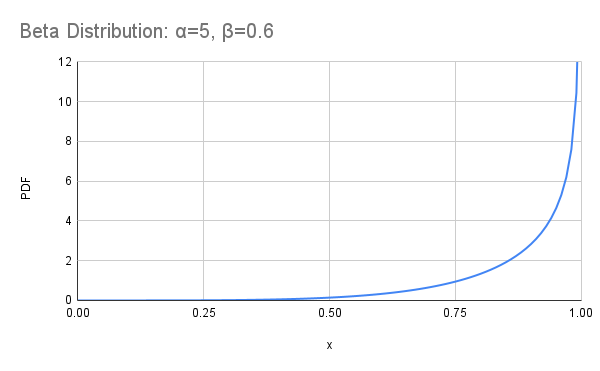
\includegraphics[scale=0.35]{media/beta.png}\end{center}
    \caption{Beta Distribution used in $\alpha\beta$-AWA*}\label{fig:beta}
\end{figure}